\usetikzlibrary{arrows.meta}
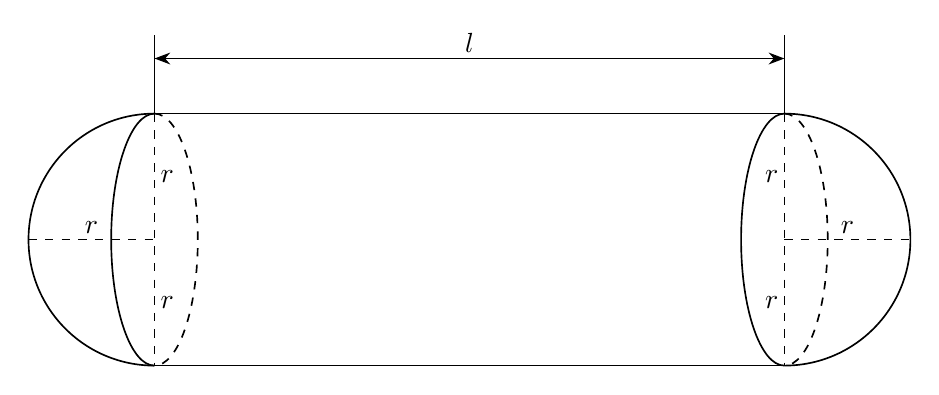
\begin{tikzpicture}[x=1cm,y=1cm,font=\normalsize,
  geometry edge/.style={draw=black,solid,line width=.6pt},
  geometry hidden/.style={draw=black,dashed,line width=.6pt},
  geometry label/.style={font=\normalsize,inner sep=2pt}]
\coordinate (CL) at (0.00,0.00);
\coordinate (CR) at (8.00,0.00);
\coordinate (LT) at (0.00,1.60);
\coordinate (LB) at (0.00,-1.60);
\coordinate (RT) at (8.00,1.60);
\coordinate (RB) at (8.00,-1.60);
\draw[geometry edge] (LT)--(RT);
\draw[geometry edge] (LB)--(RB);
\draw[geometry edge] (LT) arc (90:270:0.55 and 1.60);
\draw[geometry hidden] (LT) arc (90:-90:0.55 and 1.60);
\draw[geometry edge] (RT) arc (90:270:0.55 and 1.60);
\draw[geometry hidden] (RT) arc (90:-90:0.55 and 1.60);
\draw[geometry edge] (LT) arc (90:270:1.60 and 1.60);
\draw[geometry edge] (RT) arc (90:-90:1.60 and 1.60);
\draw[geometry hidden] (LT)--(LB);
\draw[geometry hidden] (RT)--(RB);
\draw[geometry hidden] (-1.60,0)--(CL);
\draw[geometry hidden] (CR)--(9.60,0);
\draw[geometry edge] (0.00,1.60)--(0.00,2.60);
\draw[geometry edge] (8.00,1.60)--(8.00,2.60);
\draw[geometry edge,{Stealth}-{Stealth}] (0.00,2.30)--(8.00,2.30);
\node[geometry label,above] at (4.00,2.30) {$l$};
\node[geometry label,above] at (-0.80,0.00) {$r$};
\node[geometry label,right] at (0.00,0.80) {$r$};
\node[geometry label,right] at (0.00,-0.80) {$r$};
\node[geometry label,left] at (8.00,0.80) {$r$};
\node[geometry label,left] at (8.00,-0.80) {$r$};
\node[geometry label,above] at (8.80,0.00) {$r$};
\end{tikzpicture}
